\documentclass[a4paper,12pt]{article}
\usepackage[T1]{fontenc}
\usepackage[utf8]{inputenc}
\usepackage[polish]{babel}
\usepackage{xcolor}
\usepackage{graphicx}
\usepackage{amsmath}
\usepackage{amssymb}
\usepackage{hyperref}
\usepackage{float}
\usepackage{listings}
\usepackage[backend=biber, style=numeric]{biblatex}

\addbibresource{bibliografia.bib}

\lstset{
  basicstyle=\ttfamily\small,
  columns=flexible,
  keepspaces=true,
  showstringspaces=false,
  escapeinside={(*@}{@*)},
  literate={ą}{{\k{a}}}1
           {ć}{{\'{c}}}1
           {ę}{{\k{e}}}1
           {ł}{{\l{}}}1
           {ń}{{\'{n}}}1
           {ó}{{\'{o}}}1
           {ś}{{\'{s}}}1
           {ź}{{\'{z}}}1
           {ż}{{\.{z}}}1
           {Ą}{{\k{A}}}1
           {Ć}{{\'{C}}}1
           {Ę}{{\k{E}}}1
           {Ł}{{\L{}}}1
           {Ń}{{\'{N}}}1
           {Ó}{{\'{O}}}1
           {Ś}{{\'{S}}}1
           {Ź}{{\'{Z}}}1
           {Ż}{{\.{Z}}}1
           {"}{{\textquotedbl}}1
           {'}{{\textquotesingle}}1
           {`}{{\textasciigrave}}1
           {~}{{\textasciitilde}}1
           {^}{{\textasciicircum}}1
           {_}{{\textunderscore}}1
           {|}{{\textbar}}1
           {\{}{{\textbraceleft}}1
           {\}}{{\textbraceright}}1
           {[}{{[}}1
           {]}{{]}}1,
  language=SQL,
  showspaces=false,
  numbers=left,
  numberstyle=\tiny,
  commentstyle=\color{green!60!black},
  keywordstyle=\color{blue},
  stringstyle=\color{red!80!black},
  breaklines=true, 
  frame=single,
  captionpos=b 
}

\title{5. sprawozdanie z laboratorium Hurtownie Danych}
\author{Mikołaj Kubś, 272662}
\date{\today}

\begin{document}

\maketitle

\section{Zadanie 1 - Przygotowanie powtarzalności procesu ETL}

W tym zadaniu celem było przygotowanie skryptu SQL, który umożliwi wielokrotne uruchamianie procesu ETL poprzez usunięcie istniejących tabel wymiarów, faktów oraz tabel pomocniczych, wraz z powiązanymi więzami integralności (foreign keys). Wykorzystano instrukcje `DROP TABLE IF EXISTS` oraz warunkowe usuwanie ograniczeń za pomocą `IF EXISTS` i zapytania do `INFORMATION\_SCHEMA.TABLE\_CONSTRAINTS`.

\begin{lstlisting}[caption={Skrypt SQL do usuwania obiektów bazy danych.}, label=lst:zad1_drop]
IF EXISTS (
    SELECT
        *
    FROM
        INFORMATION_SCHEMA.TABLE_CONSTRAINTS
    WHERE
        CONSTRAINT_SCHEMA = 'Kubs'
        AND CONSTRAINT_NAME = 'FK_FACT_SALES_DIM_CUSTOMER'
        AND TABLE_NAME = 'FACT_SALES'
)
ALTER TABLE
    Kubs.FACT_SALES DROP CONSTRAINT FK_FACT_SALES_DIM_CUSTOMER;

IF EXISTS (
    SELECT
        *
    FROM
        INFORMATION_SCHEMA.TABLE_CONSTRAINTS
    WHERE
        CONSTRAINT_SCHEMA = 'Kubs'
        AND CONSTRAINT_NAME = 'FK_FACT_SALES_DIM_PRODUCT'
        AND TABLE_NAME = 'FACT_SALES'
)
ALTER TABLE
    Kubs.FACT_SALES DROP CONSTRAINT FK_FACT_SALES_DIM_PRODUCT;

IF EXISTS (
    SELECT
        *
    FROM
        INFORMATION_SCHEMA.TABLE_CONSTRAINTS
    WHERE
        CONSTRAINT_SCHEMA = 'Kubs'
        AND CONSTRAINT_NAME = 'FK_FACT_SALES_DIM_SALESPERSON'
        AND TABLE_NAME = 'FACT_SALES'
)
ALTER TABLE
    Kubs.FACT_SALES DROP CONSTRAINT FK_FACT_SALES_DIM_SALESPERSON;

DROP TABLE IF EXISTS Kubs.FACT_SALES;

DROP TABLE IF EXISTS Kubs.DIM_CUSTOMER;

DROP TABLE IF EXISTS Kubs.DIM_PRODUCT;

DROP TABLE IF EXISTS Kubs.DIM_SALESPERSON;

DROP TABLE IF EXISTS Kubs.DIM_TIME;

DROP TABLE IF EXISTS Kubs.Helper_Months;

DROP TABLE IF EXISTS Kubs.Helper_Weekdays;

DROP TABLE IF EXISTS Kubs.Helper_Titles;

DROP TABLE IF EXISTS Kubs.Helper_ProductNames;
\end{lstlisting}

\section{Zadanie 2 - Wymiar czasowy}

Zadanie polegało na utworzeniu tabeli wymiaru czasu `DIM\_TIME` oraz tabel pomocniczych (`Helper\_Months`, `Helper\_Weekdays`) przechowujących polskie nazwy miesięcy i dni tygodnia. Tabela `DIM\_TIME` zawiera klucz główny w formacie RRRRMMDD oraz rozbite atrybuty daty (rok, kwartał, miesiąc, dzień miesiąca, numer dnia tygodnia) oraz ich reprezentacje słowne uzyskane przez złączenie z tabelami pomocniczymi. Dane do tabeli `DIM\_TIME` zostały wygenerowane na podstawie unikalnych dat (`OrderDate`, `ShipDate`) z tabeli `Sales.SalesOrderHeader`.

\begin{lstlisting}[caption={Tworzenie tabel pomocniczych dla wymiaru czasu.}, label=lst:zad2_helpers]
CREATE TABLE Kubs.Helper_Months (
    MonthNum INT PRIMARY KEY,
    MonthName_PL NVARCHAR(20) NOT NULL
);

INSERT INTO
    Kubs.Helper_Months (MonthNum, MonthName_PL)
VALUES
    (1, 'Styczen'),
    (2, 'Luty'),
    (3, 'Marzec'),
    (4, 'Kwiecien'),
    (5, 'Maj'),
    (6, 'Czerwiec'),
    (7, 'Lipiec'),
    (8, 'Sierpien'),
    (9, 'Wrzesien'),
    (10, 'Pazdziernik'),
    (11, 'Listopad'),
    (12, 'Grudzien');

CREATE TABLE Kubs.Helper_Weekdays (
    WeekdayNum INT PRIMARY KEY,
    WeekdayName_PL NVARCHAR(20) NOT NULL
);

INSERT INTO
    Kubs.Helper_Weekdays (WeekdayNum, WeekdayName_PL)
VALUES
    (1, 'Niedziela'),
    (2, 'Poniedzialek'),
    (3, 'Wtorek'),
    (4, 'Sroda'),
    (5, 'Czwartek'),
    (6, 'Piatek'),
    (7, 'Sobota');
\end{lstlisting}

\begin{lstlisting}[caption={Tworzenie i wypełnianie tabeli DIM\_TIME.}, label=lst:zad2_dim_time]
CREATE TABLE Kubs.DIM_TIME (
    PK_TIME INT PRIMARY KEY,
    FullDate DATE NOT NULL,
    Rok INT NOT NULL,
    Kwartal INT NOT NULL,
    Miesiac INT NOT NULL,
    Miesiac_slownie NVARCHAR(20) NOT NULL,
    Dzien_tyg INT NOT NULL,
    Dzien_tyg_slownie NVARCHAR(20) NOT NULL,
    Dzien_miesiaca INT NOT NULL
);

WITH SourceDates AS (
    SELECT
        DISTINCT OrderDate AS CalendarDate
    FROM
        Sales.SalesOrderHeader
    WHERE
        OrderDate IS NOT NULL
    UNION
    SELECT
        DISTINCT ShipDate AS CalendarDate
    FROM
        Sales.SalesOrderHeader
    WHERE
        ShipDate IS NOT NULL
)
INSERT INTO
    Kubs.DIM_TIME (
        PK_TIME,
        FullDate,
        Rok,
        Kwartal,
        Miesiac,
        Miesiac_slownie,
        Dzien_tyg,
        Dzien_tyg_slownie,
        Dzien_miesiaca
    )
SELECT
    (DATEPART(year, sd.CalendarDate) * 10000) + (DATEPART(month, sd.CalendarDate) * 100) + DATEPART(day, sd.CalendarDate) AS PK_TIME,
    sd.CalendarDate AS FullDate,
    DATEPART(year, sd.CalendarDate) AS Rok,
    DATEPART(quarter, sd.CalendarDate) AS Kwartal,
    DATEPART(month, sd.CalendarDate) AS Miesiac,
    ISNULL(hm.MonthName_PL, 'Unknown') AS Miesiac_slownie,
    DATEPART(weekday, sd.CalendarDate) AS Dzien_tygodnia,
    ISNULL(hwd.WeekdayName_PL, 'Unknown') AS Dzien_tygodnia_slownie,
    DATEPART(day, sd.CalendarDate) AS Dzien_miesiaca
FROM
    SourceDates sd
    LEFT JOIN Kubs.Helper_Months hm ON DATEPART(month, sd.CalendarDate) = hm.MonthNum
    LEFT JOIN Kubs.Helper_Weekdays hwd ON DATEPART(weekday, sd.CalendarDate) = hwd.WeekdayNum;
\end{lstlisting}

\begin{figure}[H]
    \centering
    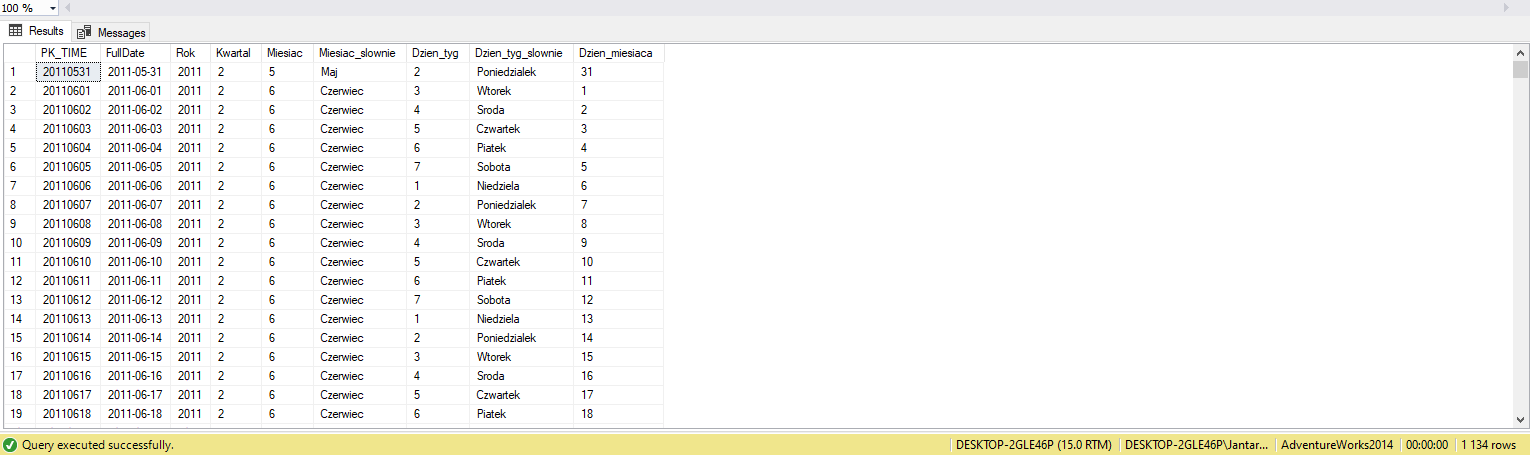
\includegraphics[width=0.8\textwidth]{images/2_time_rows.png}
    \caption{Przykładowe dane w tabeli Kubs.DIM\_TIME.}
    \label{fig:dim_time_data}
\end{figure}

\section{Zadanie 3 - Elementarne czyszczenie danych}

Celem tego zadania było zaimplementowanie podstawowego mechanizmu czyszczenia danych podczas procesu ładowania wymiarów. Polegało to na zastąpieniu wartości NULL w określonych kolumnach (`Color`, `SubCategoryName` w `DIM\_PRODUCT`; `CountryRegionCode`, `Group` w `DIM\_CUSTOMER` i `DIM\_SALESPERSON`) predefiniowanymi wartościami domyślnymi ('Unknown', '000'). Zastosowano funkcję `ISNULL()` podczas procesu INSERT danych.

\begin{lstlisting}[caption={Przykład czyszczenia danych w instrukcji SELECT.}, label=lst:zad3_cleanse_example]
    INSERT INTO
    Kubs.DIM_CUSTOMER (
        CustomerID,
        FirstName,
        LastName,
        Title,
        City,
        TerritoryName,
        CountryRegionCode,
        [Group]
    )
SELECT
    c.CustomerID,
    MIN(p.FirstName) AS FirstName,
    MIN(p.LastName) AS LastName,
    MIN(p.Title) AS Title,
    MIN(a.City) AS City,
    MIN(st.Name) AS TerritoryName,
    -- zmiana tutaj
    ISNULL(MIN(st.CountryRegionCode), '000') AS CountryRegionCode,
    ISNULL(MIN(st.[Group]), 'Unknown') AS [Group]
    -- zmiana tutaj
FROM
    Sales.Customer AS c
    LEFT JOIN Person.Person AS p ON c.PersonID = p.BusinessEntityID
    LEFT JOIN Sales.SalesTerritory AS st ON c.TerritoryID = st.TerritoryID
    LEFT JOIN Person.BusinessEntityAddress bea ON p.BusinessEntityID = bea.BusinessEntityID
    LEFT JOIN Person.Address AS a ON bea.AddressID = a.AddressID
WHERE
    c.PersonID IS NOT NULL
GROUP BY
    c.CustomerID;

INSERT INTO
    Kubs.DIM_PRODUCT (
        ProductID,
        Name,
        ListPrice,
        Color,
        SubCategoryName,
        CategoryName,
        Weight,
        Size
    )
SELECT
    DISTINCT p.ProductID,
    p.Name,
    p.ListPrice,
    -- zmiana tutaj
    ISNULL(p.Color, 'Unknown') AS Color,
    ISNULL(psc.Name, 'Unknown') AS SubCategoryName,
    -- zmiana tutaj
    pc.Name AS CategoryName,
    p.Weight,
    p.Size
FROM
    Production.Product AS p
    INNER JOIN Sales.SalesOrderDetail AS sod ON p.ProductID = sod.ProductID
    LEFT JOIN Production.ProductSubcategory AS psc ON p.ProductSubcategoryID = psc.ProductSubcategoryID
    LEFT JOIN Production.ProductCategory AS pc ON psc.ProductCategoryID = pc.ProductCategoryID;

INSERT INTO
    Kubs.DIM_SALESPERSON (
        SalesPersonID,
        FirstName,
        LastName,
        Title,
        Gender,
        CountryRegionCode,
        [Group]
    )
SELECT
    sp.BusinessEntityID AS SalesPersonID,
    p.FirstName,
    p.LastName,
    p.Title,
    e.Gender,
    -- zmiana tutaj
    ISNULL(st.CountryRegionCode, '000') AS CountryRegionCode,
    ISNULL(st.[Group], 'Unknown') AS [Group]
    -- zmiana tutaj
FROM
    Sales.SalesPerson AS sp
    INNER JOIN Person.Person AS p ON sp.BusinessEntityID = p.BusinessEntityID
    INNER JOIN HumanResources.Employee AS e ON sp.BusinessEntityID = e.BusinessEntityID
    LEFT JOIN Sales.SalesTerritory AS st ON sp.TerritoryID = st.TerritoryID;

INSERT INTO
    Kubs.FACT_SALES (
        ProductID,
        CustomerID,
        SalesPersonID,
        OrderDate,
        ShipDate,
        OrderQty,
        UnitPrice,
        UnitPriceDiscount,
        LineTotal
    )
SELECT
    sod.ProductID,
    soh.CustomerID,
    soh.SalesPersonID,
    DATEPART(YEAR, soh.OrderDate) * 10000 + DATEPART(MONTH, soh.OrderDate) * 100 + DATEPART(DAY, soh.OrderDate) AS OrderDate,
    DATEPART(YEAR, soh.ShipDate) * 10000 + DATEPART(MONTH, soh.ShipDate) * 100 + DATEPART(DAY, soh.ShipDate) AS ShipDate,
    sod.OrderQty,
    sod.UnitPrice,
    sod.UnitPriceDiscount,
    sod.LineTotal
FROM
    Sales.SalesOrderDetail AS sod
    INNER JOIN Sales.SalesOrderHeader AS soh ON sod.SalesOrderID = soh.SalesOrderID;
\end{lstlisting}

\section{Zadanie 4 - Proces Extact - Transform - Load (SQL)}

W tym zadaniu zautomatyzowano proces ETL z poprzednich kroków (oraz z Laboratorium 4) za pomocą pakietu SSIS (SQL Server Integration Services). Wykorzystano wyłącznie komponenty `Execute SQL Task` w zakładce `Control Flow` do wykonania kolejnych kroków:
\begin{enumerate}
    \item Usunięcie istniejących obiektów (skrypt z zadania 1).
    \item Utworzenie struktur tabel wymiarów, faktów i pomocniczych (skrypt z zadania 2).
    \item Wypełnienie tabel wymiarów (DIM\_TIME, DIM\_CUSTOMER, DIM\_PRODUCT, DIM\_SALESPERSON) wyczyszczonymi danymi.
    \item Wypełnienie tabeli faktów (FACT\_SALES) danymi zagregowanymi i kluczami obcymi.
    \item Dodanie więzów integralności.
    \item Dodano obsługę błędów (Event Handlers)
    \item Dodano powiadomienie o sukcesie (skrypt C\#).
\end{enumerate}

\begin{lstlisting}[caption={Dodanie nowych CONSTRAINT}]
-- poprzednie wiersze z poprzedniej listy...
ALTER TABLE
    Kubs.FACT_SALES WITH NOCHECK
ADD
    CONSTRAINT FK_FACT_SALES_DIM_TIME_OrderDate FOREIGN KEY (OrderDate) REFERENCES Kubs.DIM_TIME(PK_TIME);

GO
ALTER TABLE
    Kubs.FACT_SALES WITH NOCHECK
ADD
    CONSTRAINT FK_FACT_SALES_DIM_TIME_ShipDate FOREIGN KEY (ShipDate) REFERENCES Kubs.DIM_TIME(PK_TIME);
\end{lstlisting}

\begin{figure}[H]
    \centering
    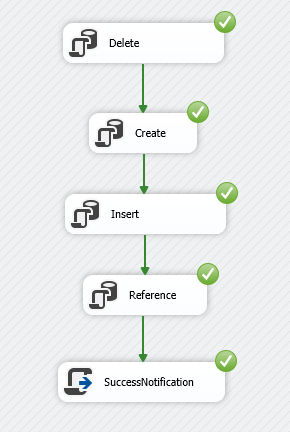
\includegraphics[width=0.5\textwidth]{images/4_success_2.png}
    \caption{Schemat Control Flow pakietu SSIS realizującego ETL za pomocą Execute SQL Task.}
    \label{fig:zad4_control_flow_2}
\end{figure}

\begin{figure}[H]
    \centering
    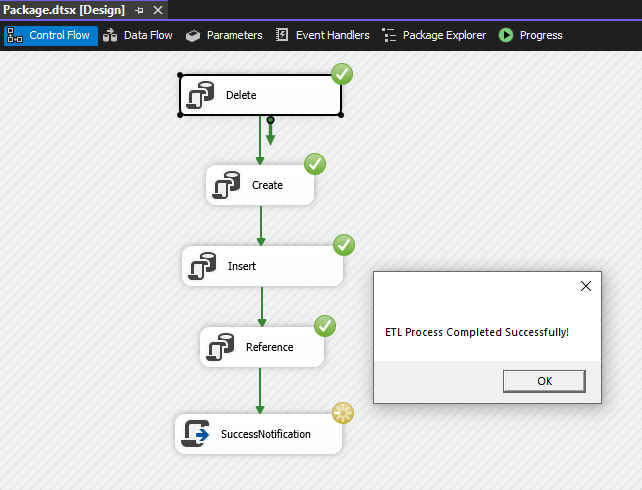
\includegraphics[width=0.5\textwidth]{images/4_success.png}
    \caption{Komunikat oznajmiający sukces załadowania danych.}
    \label{fig:zad4_control_flow}
\end{figure}

\begin{figure}[H]
    \centering
    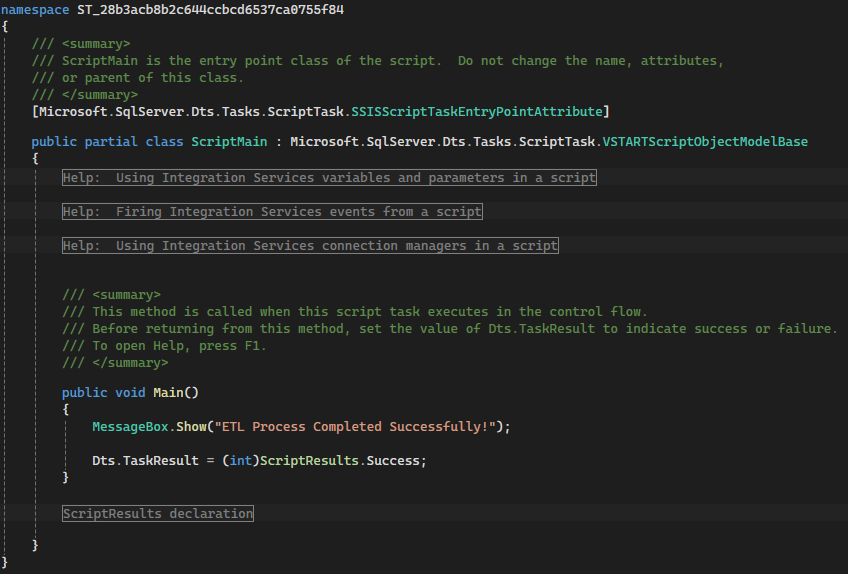
\includegraphics[width=0.5\textwidth]{images/4_script.png}
    \caption{Skrypt odpowiedzialny za oznajmienie sukcesu.}
    \label{fig:zad4_script}
\end{figure}

\section{Zadanie 5 - ETL (prawie) bez SQLa (Data Flow)}

Zadanie 5 polegało na refaktoryzacji procesu ETL z zadania 4, tak aby ładowanie danych do wymiaru czasu (`DIM\_TIME`) oraz co najmniej jednego innego wybranego wymiaru (np. `DIM\_PRODUCT`) odbywało się przy użyciu komponentów graficznych z zakładki `Data Flow` w SSIS, minimalizując użycie bezpośrednich zapytań SQL w tych krokach. Wykorzystano m.in.:
\begin{itemize}
    \item `OLE DB Source`: Do pobierania danych ze źródłowych tabel AdventureWorks.
    \item `Derived Column`: Do tworzenia nowych kolumn (np. `PK\_TIME`, `Rok`, `Kwartał`), implementacji czyszczenia danych (`ISNULL(Color, 'Unknown')`).
          *   `Union All`: Do połączenia strumieni danych (np. OrderDate i ShipDate).
          *   `Conditional Split`: Do filtrowania (np. usuwania NULLi).
    \item `Lookup`: Do wzbogacania danych poprzez dołączanie informacji z innych tabel (np. nazw miesięcy/dni tygodnia z tabel pomocniczych, nazw kategorii/podkategorii produktów, danych osobowych, terytoriów). Użyto różnych trybów cache'owania.
          *   `Sort`: Do sortowania danych, a w szczególności do usuwania duplikatów (np. dla `DIM\_CUSTOMER` w celu zapewnienia unikalności `CustomerID`).
          *   `Fuzzy Grouping` / `Fuzzy Lookup`: (Opcjonalnie, jeśli były używane do analizy lub czyszczenia np. nazw produktów).
    \item `OLE DB Destination`: Do zapisywania przetworzonych danych do docelowych tabel w schemacie `Kubs`, często w trybie `Fast Load`.
\end{itemize}
Pozostałe kroki, jak usuwanie i tworzenie tabel oraz dodawanie ograniczeń, mogły pozostać realizowane przez `Execute SQL Task`.

% --- POCZĄTEK MIEJSCA NA OBRAZKI ZADANIA 5 ---
\begin{figure}[H]
    \centering
    % \includegraphics[width=\textwidth]{sciezka/do/obrazka_zad5_dft_dim_time.png} % Odkomentuj i podaj ścieżkę
    \fbox{(*@\textit{Tutaj wstaw rysunek przedstawiający Data Flow Task dla DIM\_TIME}@*)}
    \caption{Schemat Data Flow Task dla ładowania wymiaru czasu (DIM\_TIME).}
    \label{fig:zad5_dft_dim_time}
\end{figure}

\begin{figure}[H]
    \centering
    % \includegraphics[width=\textwidth]{sciezka/do/obrazka_zad5_dft_inny_wymiar.png} % Odkomentuj i podaj ścieżkę
    \fbox{(*@\textit{Tutaj wstaw rysunek przedstawiający Data Flow Task dla drugiego wybranego wymiaru (np. DIM\_PRODUCT lub DIM\_CUSTOMER)}@*)}
    \caption{Schemat Data Flow Task dla ładowania wybranego innego wymiaru.}
    \label{fig:zad5_dft_other_dim}
\end{figure}

% (Opcjonalnie) Rysunek całego Control Flow dla Zadania 5
\begin{figure}[H]
    \centering
    % \includegraphics[width=0.9\textwidth]{sciezka/do/obrazka_zad5_control_flow.png} % Odkomentuj i podaj ścieżkę
    \fbox{(*@\textit{Tutaj wstaw rysunek przedstawiający Control Flow pakietu SSIS z Zadania 5 (z użyciem Data Flow Task)}@*)}
    \caption{Schemat Control Flow pakietu SSIS wykorzystującego Data Flow Task.}
    \label{fig:zad5_control_flow}
\end{figure}
% --- KONIEC MIEJSCA NA OBRAZKI ZADANIA 5 ---

\section{Wnioski}

 % Tutaj napisz swoje wnioski z laboratorium 5.
 % - Podsumuj wykonane zadania.
 % - Jakie były główne wyzwania? (np. konfiguracja DFT, logika lookupów, de-duplikacja)
 % - Porównaj podejście z Zadania 4 (tylko SQL) z podejściem z Zadania 5 (Data Flow). Jakie są zalety i wady każdego z nich w kontekście tego laboratorium? (np. czytelność, wydajność, łatwość modyfikacji, złożoność implementacji).
 % - Czy napotkałeś jakieś problemy podczas implementacji Fuzzy Grouping/Lookup (jeśli próbowałeś)?
 % - Jakie są korzyści z posiadania wymiaru czasu?
 % - Znaczenie powtarzalności procesu ETL.
 (*@\textit{W tym miejscu wpisz swoje przemyślenia i wnioski dotyczące wykonanych zadań.}@*)


% Jeśli korzystałeś z zewnętrznych źródeł oprócz podanych w instrukcji, dodaj je do pliku bibliografia.bib i odwołaj się do nich w tekście za pomocą \cite{klucz_bib}
% np. Dodatkowe informacje na temat Fuzzy Grouping można znaleźć w \cite{przyklad_online}.

\printbibliography

\end{document}